%==============================================================================
% DISSERTATION PROGRESS REPORT
% Formal-Informal Linkages in Indian Textiles & Apparel
% Beamer Presentation — February 2026
%==============================================================================

\documentclass[aspectratio=169, 10pt]{beamer}

%--- Theme & Colours ----------------------------------------------------------
\usetheme{Madrid}
\usecolortheme{default}

% Custom colour palette: deep blue + gold accent
\definecolor{darkblue}{RGB}{15, 40, 90}
\definecolor{gold}{RGB}{200, 160, 30}
\definecolor{lightgray}{RGB}{240, 240, 245}
\definecolor{deepred}{RGB}{160, 30, 30}
\definecolor{teal}{RGB}{0, 120, 120}

\setbeamercolor{palette primary}{bg=darkblue, fg=white}
\setbeamercolor{palette secondary}{bg=darkblue!85, fg=white}
\setbeamercolor{palette tertiary}{bg=darkblue!70, fg=white}
\setbeamercolor{palette quaternary}{bg=darkblue, fg=white}
\setbeamercolor{frametitle}{bg=darkblue, fg=white}
\setbeamercolor{title}{bg=darkblue, fg=white}
\setbeamercolor{structure}{fg=darkblue}
\setbeamercolor{block title}{bg=darkblue, fg=white}
\setbeamercolor{block body}{bg=lightgray}
\setbeamercolor{alerted text}{fg=gold}
\setbeamercolor{example text}{fg=teal}

%--- Fonts --------------------------------------------------------------------
\usefonttheme{professionalfonts}
\setbeamerfont{title}{size=\large, series=\bfseries}
\setbeamerfont{frametitle}{size=\normalsize, series=\bfseries}

%--- Outer theme adjustments --------------------------------------------------
\setbeamertemplate{navigation symbols}{}   % remove nav icons
\setbeamertemplate{footline}{%
  \leavevmode%
  \hbox{%
    \begin{beamercolorbox}[wd=.35\paperwidth,ht=2.25ex,dp=1ex,left,leftskip=1em]{palette primary}%
      \usebeamerfont{author in head/foot}\insertshortauthor
    \end{beamercolorbox}%
    \begin{beamercolorbox}[wd=.38\paperwidth,ht=2.25ex,dp=1ex,center]{palette secondary}%
      \usebeamerfont{title in head/foot}\insertshorttitle
    \end{beamercolorbox}%
    \begin{beamercolorbox}[wd=.27\paperwidth,ht=2.25ex,dp=1ex,right,rightskip=1em]{palette primary}%
      \usebeamerfont{date in head/foot}February 2026\hspace{1em}%
      \insertframenumber{} / \inserttotalframenumber
    \end{beamercolorbox}}%
}

%--- Packages -----------------------------------------------------------------
\usepackage{booktabs}
\usepackage{amsmath}
\usepackage{graphicx}
\usepackage{xcolor}
\usepackage{tikz}
\usepackage{array}
\usepackage{multirow}
\usepackage[T1]{fontenc}
\usepackage{lmodern}

%--- Helpers ------------------------------------------------------------------
\newcommand{\yes}{\textcolor{teal}{\textbf{Yes}}}
\newcommand{\no}{\textcolor{deepred}{\textbf{No}}}
\newcommand{\key}[1]{\textcolor{gold}{\textbf{#1}}}
\newcommand{\sig}[1]{\textcolor{teal}{\textbf{#1}}}
\newcommand{\ins}[1]{\textcolor{gray}{#1}}

%==============================================================================
\title[Formal-Informal Linkages: Progress Report]{%
  Formal-Informal Linkages in Indian Textiles \& Apparel\\[4pt]
  \small Dissertation Progress Report --- Stage 1 Analysis}
\author[Ashwin Sreekumar]{Ashwin Sreekumar}
\institute{Dissertation Progress Presentation}
\date{February 20, 2026}
%==============================================================================

\begin{document}

%--- Title Slide --------------------------------------------------------------
\begin{frame}
\titlepage
\end{frame}

%--- Outline ------------------------------------------------------------------
\begin{frame}{Outline}
\tableofcontents
\end{frame}

%==============================================================================
\section{Research Questions \& Theoretical Framework}
%==============================================================================

\begin{frame}{Research Questions}
\begin{block}{Core Hypothesis}
Formal sector productivity \textbf{spills over} to the informal sector through two channels:
informal wages and strategic outsourcing (job work).
\end{block}

\bigskip
\begin{columns}[T]
\begin{column}{0.48\textwidth}
  \textbf{RQ1: Wage Pass-Through}\\[4pt]
  Does higher formal sector productivity raise informal sector wages?\\[8pt]
  \[
    \ln w^{inf}_{si} = \alpha + \beta \ln A^{f}_{si} + \varepsilon_{si}
  \]
\end{column}
\begin{column}{0.48\textwidth}
  \textbf{RQ2: Strategic Outsourcing}\\[4pt]
  Does formal sector productivity drive outsourcing intensity to informal job-work firms?\\[8pt]
  \[
    \ln Q^{out}_{si} = \alpha + \gamma \ln A^{f}_{si} + \varepsilon_{si}
  \]
\end{column}
\end{columns}

\bigskip
\begin{alertblock}{RQ3: Enforcement Moderation}
  \centering
  Does labor law enforcement $E_s$ moderate these linkages across states?
\end{alertblock}
\end{frame}

%------------------------------------------------------------------------------
\begin{frame}{Theoretical Mechanism}
\begin{center}
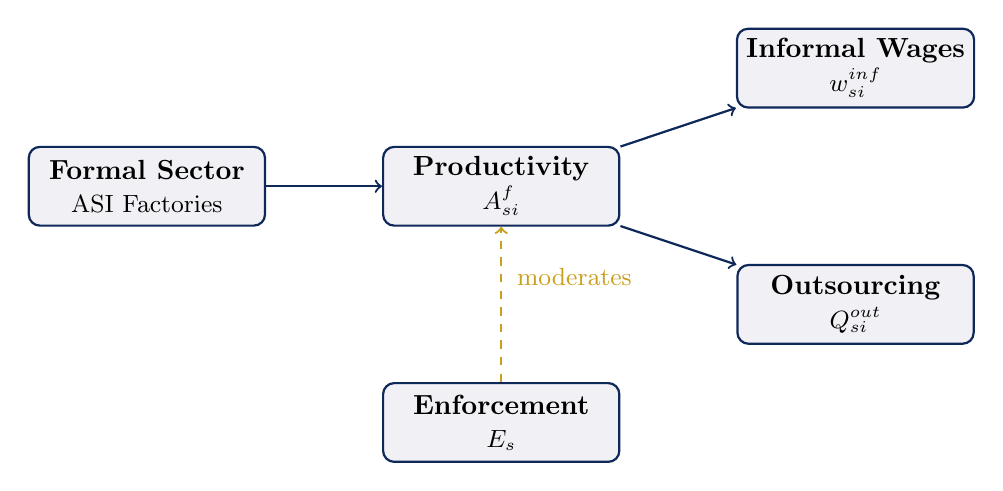
\begin{tikzpicture}[
  box/.style={rectangle, draw=darkblue, thick, rounded corners=4pt,
              minimum width=3cm, minimum height=1cm, align=center,
              fill=lightgray},
  arr/.style={->, thick, darkblue},
  mod/.style={->, thick, gold, dashed}
]

\node[box] (formal) at (0,0) {\textbf{Formal Sector}\\\small ASI Factories};
\node[box] (prod)   at (4.5,0) {\textbf{Productivity}\\\small $A^f_{si}$};
\node[box] (wages)  at (9, 1.5) {\textbf{Informal Wages}\\\small $w^{inf}_{si}$};
\node[box] (out)    at (9,-1.5) {\textbf{Outsourcing}\\\small $Q^{out}_{si}$};
\node[box] (enf)    at (4.5,-3) {\textbf{Enforcement}\\\small $E_s$};

\draw[arr] (formal) -- (prod);
\draw[arr] (prod) -- (wages);
\draw[arr] (prod) -- (out);
\draw[mod] (enf) -- node[right, xshift=2pt, yshift=10pt]
           {\textcolor{gold}{\small moderates}} (prod);

\end{tikzpicture}
\end{center}

\vspace{6pt}
\small
\textbf{Context:} India's Textiles (NIC-13) \& Apparel (NIC-14) sectors are deeply integrated —
large formal factories outsource labour-intensive tasks to millions of small informal ``job work'' enterprises.
\end{frame}

%==============================================================================
\section{Data \& Methodology}
%==============================================================================

\begin{frame}{Data Sources}
\begin{columns}[T]
\begin{column}{0.48\textwidth}
  \begin{block}{Formal Sector --- ASI 2023--24}
    \textit{Annual Survey of Industries}
    \begin{itemize}
      \item \textbf{68,641} total factories
      \item \textbf{8,137} textiles \& apparel factories
      \item 33 states with usable data
      \item Key variables: output (Block J), employment (Block E), outsourcing cost (Block F)
    \end{itemize}
  \end{block}
\end{column}
\begin{column}{0.48\textwidth}
  \begin{block}{Informal Sector --- ASUSE 2023--24}
    \textit{Annual Survey of Unincorporated Sector Enterprises}
    \begin{itemize}
      \item \textbf{144,910} unique enterprises
      \item \textbf{7,519} job-work enterprises\\ (textiles \& apparel)
      \item Key filter: \texttt{contract\_manuf\_service=1}
      \item Key variables: hired workers (Item 511), wages (Item 559)
    \end{itemize}
  \end{block}
\end{column}
\end{columns}

\vspace{8pt}
\begin{exampleblock}{Enforcement Data --- $E_s$}
  Inspections-to-factories ratio per state. Source: DGFASLI Standard Reference Note (SRN) 2023.\\
  $E_s = \text{Total Inspections} / \text{Working Factories}$ \hfill Range: $[0, 1]$, Mean = 0.22, SD = 0.196
\end{exampleblock}
\end{frame}

%------------------------------------------------------------------------------
\begin{frame}{Key Methodological Choices (and Why)}
\begin{columns}[T]
\begin{column}{0.55\textwidth}
  \begin{block}{Analysis Level: State $\times$ Industry}
  \begin{itemize}
    \item \textbf{Original plan:} District--Industry
    \item \textbf{Constraint:} Public ASI data suppresses all district/state geo-codes for confidentiality
    \item \textbf{Solution:} Use state codes from ASI field \texttt{a7}; ASUSE \texttt{district} field maps to states
    \item \textbf{Justification:} Enforcement is a state-level policy — state analysis is theoretically natural
  \end{itemize}
  \end{block}
\end{column}
\begin{column}{0.42\textwidth}
  \begin{alertblock}{Data Limitation (Documented)}
  \begin{itemize}
    \item No district-level analysis possible from public data
    \item MOSPI restricted-access data would enable district IDs (3--6 month wait)
    \item This limitation narrows to N=47 obs
  \end{itemize}
  \end{alertblock}

  \medskip
  \begin{block}{Job Work Definition}
  \texttt{contract\_manuf\_service = 1}\\[4pt]
  $\Rightarrow$ 7,519 enterprises\\
  (vs.\ only 30 using \texttt{nature\_of\_operation=3})
  \end{block}
\end{column}
\end{columns}
\end{frame}

%------------------------------------------------------------------------------
\begin{frame}{Variable Construction}
\begin{table}
\centering
\small
\renewcommand{\arraystretch}{1.35}
\begin{tabular}{@{}p{3.2cm} p{4.5cm} p{4.8cm}@{}}
\toprule
\textbf{Variable} & \textbf{Construction} & \textbf{Source Field} \\
\midrule
\multicolumn{3}{l}{\textit{Formal Sector (ASI)}} \\
$A^f_{si}$ — Productivity & Output / Employment & J113 / (EI7/300) \\
$Q^{out}_{si}$ — Outsourcing & Contract cost / Output & F7 / J113 \\
$L^f_{si}$ — Employment & $\sum(\text{mandays})/300$ & EI7 \\
\midrule
\multicolumn{3}{l}{\textit{Informal Sector (ASUSE)}} \\
$w^{inf}_{si}$ — Avg. Wage & Total wages / Hired workers & Item 559 / Item 511 \\
\midrule
\multicolumn{3}{l}{\textit{Enforcement}} \\
$E_s$ — Enforcement & Inspections / Working factories & MoLE Annual Report \\
\midrule
\multicolumn{3}{l}{\textit{Aggregation}} \\
State--Industry & Weighted mean (multiplier weights) & ASI: \texttt{mult}; ASUSE: \texttt{mlt} \\
Winsorization & 1\% -- 99\% & All log-transformed variables \\
\bottomrule
\end{tabular}
\end{table}
\end{frame}

%------------------------------------------------------------------------------
\begin{frame}{Regression Models}
\begin{block}{Model 1 --- Wage Pass-Through with Enforcement Interaction}
\[
\ln w^{inf}_{si} = \alpha + \beta_1 E_s + \beta_2 \ln A^f_{si} + \beta_3 \left(E_s \times \ln A^f_{si}\right) + \mu_i + \varepsilon_{si}
\]
\end{block}

\bigskip

\begin{block}{Model 2 --- Strategic Outsourcing with Enforcement}
\[
\ln Q^{out}_{si} = \alpha + \delta_1 E_s + \delta_2 E_s^2 + \delta_3 \ln A^f_{si} + \mu_i + \varepsilon_{si}
\]
\end{block}

\bigskip
\begin{columns}[T]
\begin{column}{0.48\textwidth}
  \small
  \begin{itemize}
    \item $\mu_i$ = 2-digit NIC fixed effects (absorbs industry-level differences)
    \item Standard errors clustered at state level
    \item $E_s^2$ term tests for non-linear (inverted-U) enforcement effect
  \end{itemize}
\end{column}
\begin{column}{0.48\textwidth}
  \small
  \begin{itemize}
    \item \textbf{Sample}: 47 state--industry cells, 26 states, 2 industries
    \item \textbf{Industries}: NIC-13 (Textiles), NIC-14 (Apparel)
    \item \textbf{Estimator}: OLS with high-dim fixed effects (\texttt{fixest} package)
  \end{itemize}
\end{column}
\end{columns}
\end{frame}

%==============================================================================
\section{Sample \& Descriptive Statistics}
%==============================================================================

\begin{frame}{Sample Construction Summary}
\begin{center}
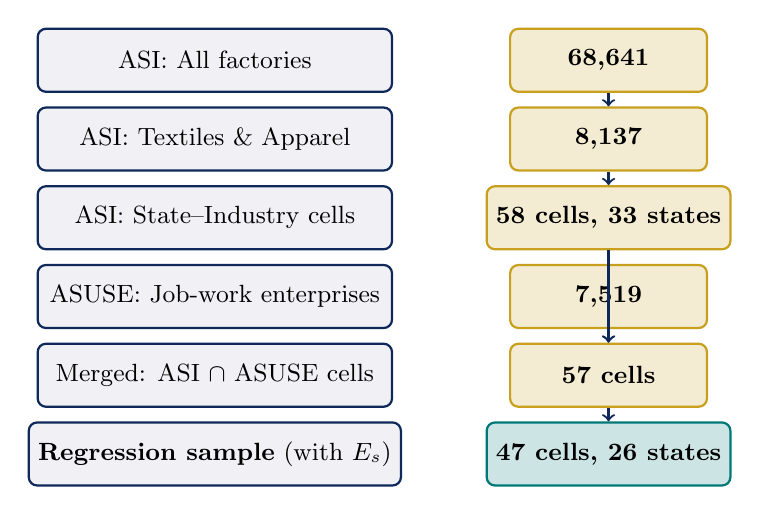
\begin{tikzpicture}[
  stage/.style={rectangle, draw=darkblue, thick, rounded corners=3pt,
                minimum width=4.5cm, minimum height=0.8cm, align=center,
                fill=lightgray, font=\small},
  num/.style={rectangle, draw=gold, thick, rounded corners=3pt,
              minimum width=2.5cm, minimum height=0.8cm, align=center,
              fill=gold!20, font=\small\bfseries},
  arr/.style={->, thick, darkblue}
]

\node[stage] (a1) at (0,4)    {ASI: All factories};
\node[num]   (n1) at (5,4)    {68,641};

\node[stage] (a2) at (0,3)    {ASI: Textiles \& Apparel};
\node[num]   (n2) at (5,3)    {8,137};

\node[stage] (a3) at (0,2)    {ASI: State--Industry cells};
\node[num]   (n3) at (5,2)    {58 cells, 33 states};

\node[stage] (b1) at (0,1)    {ASUSE: Job-work enterprises};
\node[num]   (b2) at (5,1)    {7,519};

\node[stage] (c1) at (0,0)    {Merged: ASI $\cap$ ASUSE cells};
\node[num]   (c2) at (5,0)    {57 cells};

\node[stage] (d1) at (0,-1)   {\textbf{Regression sample} (with $E_s$)};
\node[num,fill=teal!20,draw=teal]
             (d2) at (5,-1)   {\textbf{47 cells, 26 states}};

\draw[arr] (n1) -- (n2);
\draw[arr] (n2) -- (n3);
\draw[arr] (n3) -- (c2);
\draw[arr] (b2) -- (c2);
\draw[arr] (c2) -- (d2);

\end{tikzpicture}
\end{center}
\end{frame}

%------------------------------------------------------------------------------
\begin{frame}{Descriptive Statistics}
\begin{table}
\centering
\small
\renewcommand{\arraystretch}{1.3}
\begin{tabular}{@{}lrrrrr@{}}
\toprule
\textbf{Variable} & \textbf{N} & \textbf{Mean} & \textbf{Median} & \textbf{Std. Dev.} & \textbf{Range} \\
\midrule
$\ln w^{inf}_{si}$ (Informal wage, log) & 47 & 3.394 & 3.445 & 0.457 & [2.33, 4.09] \\
$\ln A^f_{si}$ (Formal productivity, log) & 47 & 13.85 & 14.00 & 0.895 & [10.42, 15.44] \\
$\ln Q^{out}_{si}$ (Outsourcing share, log) & 47 & $\approx0$ & 0 & --- & [0, $3.9\times10^{-5}$] \\
$E_s$ (Enforcement ratio) & 47 & 0.223 & 0.165 & 0.196 & [0.00, 1.00] \\
\midrule
$N^{firms}$ (ASI factories per cell) & 47 & 98.7 & 20 & --- & [1, 905] \\
$N^{inf}$ (ASUSE enterprises per cell) & 47 & 84.5 & 57 & --- & [1, 305] \\
\bottomrule
\end{tabular}
\smallskip
\end{table}

\begin{columns}[T]
\begin{column}{0.48\textwidth}
\begin{exampleblock}{Enforcement Variation}
  \textbf{Low enforcement}: Chandigarh (0), Uttarakhand (0.018), Bihar (0.014)\\
  \textbf{High enforcement}: J\&K (0.654), Karnataka (0.403), Gujarat (0.477)\\
  \textbf{Outlier}: Manipur ($E_s = 1.0$)
\end{exampleblock}
\end{column}
\begin{column}{0.48\textwidth}
\begin{block}{Key Correlations}
  \begin{tabular}{lrr}
    & $\ln A^f$ & $E_s$ \\
    \midrule
    $\ln w^{inf}$ & $-0.032$ & $-0.281$ \\
    $\ln Q^{out}$ & $\mathbf{+0.285}$ & $-0.011$ \\
  \end{tabular}
\end{block}
\end{column}
\end{columns}
\end{frame}

%==============================================================================
\section{Regression Results}
%==============================================================================

\begin{frame}{Main Regression Results}
\begin{table}
\centering
\small
\renewcommand{\arraystretch}{1}
\begin{tabular}{@{}lcc@{}}
\toprule
 & \textbf{Model 1} & \textbf{Model 2} \\
 & $\ln w^{inf}_{si}$ & $\ln Q^{out}_{si}$ \\
\midrule
$E_s$ & \ins{0.114} & \ins{$6.75 \times 10^{-6}$} \\
      & \ins{(5.087)} & \ins{($1.39 \times 10^{-5}$)} \\[4pt]
$\ln A^f_{si}$ & \ins{$-0.029$} & \sig{$3.72 \times 10^{-6}$\,*} \\
               & \ins{(0.072)} & \sig{($1.74 \times 10^{-6}$)} \\[4pt]
$E_s \times \ln A^f_{si}$ & \ins{$-0.059$} & --- \\
                           & \ins{(0.378)} & \\[4pt]
$E_s^2$ & --- & \ins{$-4.26 \times 10^{-6}$} \\
        & & \ins{($1.25 \times 10^{-5}$)} \\
\midrule
NIC Fixed Effects & \yes & \yes \\
S.E.\ Clustered (State) & \yes & \yes \\
Observations & 47 & 47 \\
Within $R^2$ & 0.081 & \textbf{0.102} \\
\bottomrule
\multicolumn{3}{l}{\small * $p<0.05$;\quad Standard errors in parentheses.\quad Grey = not significant.}
\end{tabular}
\end{table}
\end{frame}

%------------------------------------------------------------------------------
\begin{frame}{Interpreting the Results}

\begin{columns}[T]
\begin{column}{0.48\textwidth}
  \begin{alertblock}{Model 1 --- Wage Pass-Through \textit{(Not Significant)}}
    \begin{itemize}
      \item No significant positive pass-through of formal productivity to informal wages
      \item Enforcement does not significantly moderate the wage channel ($p>0.87$)
      \item \textbf{Why?} Small N~(47 obs), cross-sectional data lack time variation
      \item \textbf{Direction}: Negative $\beta_2=-0.029$ may reflect labour market segmentation
    \end{itemize}
  \end{alertblock}
\end{column}
\begin{column}{0.4\textwidth}
  \begin{exampleblock}{Model 2 --- Outsourcing \textit{(Significant!)} $p=0.043$}
    \begin{itemize}
      \item \textbf{Formal productivity significantly increases outsourcing intensity}
      \item $\hat\delta_3 = 3.72 \times 10^{-6}$, $t=2.14$, $p=0.043$
      \item Higher-productivity formal firms outsource \emph{more} to informal job-work enterprises
      \item \textbf{Consistent with} value-chain specialisation hypothesis
      \item $E_s$ terms not significant --- enforcement doesn't deter outsourcing on its own
    \end{itemize}
  \end{exampleblock}
\end{column}
\end{columns}

\bigskip
\begin{block}{Bottom Line}
  \centering
  \key{Higher formal sector productivity $\rightarrow$ more outsourcing to informal sector} (\textit{significant})\\
  Wage spillover channel not yet confirmed at state level
\end{block}

\end{frame}

%------------------------------------------------------------------------------
\begin{frame}{Enforcement \& Informal Wages: Correlation Evidence}

\begin{columns}[T]
\begin{column}{0.55\textwidth}
  \begin{block}{Raw Correlation: $E_s$ \& $\ln w^{inf}$}
    \[
      \text{corr}(E_s,\, \ln w^{inf}) = -0.281
    \]
    \begin{itemize}
      \item States with \textbf{stricter enforcement} tend to have \textbf{lower informal wages}
      \item Consistent with enforcement raising barriers for informal firms
      \item Informal firms pay less when they cannot absorb compliance costs
      \item Not causal — omitted state characteristics may explain this
    \end{itemize}
  \end{block}
\end{column}
\begin{column}{0.42\textwidth}
  \begin{table}
  \small
  \renewcommand{\arraystretch}{1.25}
  \begin{tabular}{@{}lrr@{}}
  \toprule
  \textbf{State} & $E_s$ & $\ln w^{inf}$ \\
  \midrule
  Gujarat & 0.477 & $\sim$3.1 \\
  Karnataka & 0.403 & $\sim$3.3 \\
  Tamil Nadu & 0.313 & $\sim$3.5 \\
  Haryana & 0.103 & $\sim$3.7 \\
  Uttarakhand & 0.018 & $\sim$4.1 \\
  \bottomrule
  \multicolumn{3}{l}{\tiny Illustrative values from regression sample}
  \end{tabular}
  \end{table}
  \vspace{4pt}
  \textit{Higher $E_s$ \textbf{\textcolor{deepred}{$\downarrow$}} waged}
\end{column}
\end{columns}

\end{frame}

%==============================================================================
\section{Limitations \& Next Steps}
%==============================================================================

\begin{frame}{Limitations}
\begin{columns}[T]
\begin{column}{0.48\textwidth}
  \begin{alertblock}{Data \& Geographic Constraints}
    \begin{enumerate}
      \item \textbf{Small N}: Only 47 state--industry observations reduces statistical power
      \item \textbf{Cross-sectional}: Single year (2023--24) — no panel variation
      \item \textbf{ASI geography suppressed}: District codes unavailable in public unit-level data
      \item \textbf{6 states missing} enforcement records (HP, UP, WB, Arunachal, Daman~\&~Diu)
    \end{enumerate}
  \end{alertblock}
\end{column}
\begin{column}{0.48\textwidth}
  \begin{block}{Methodological Notes}
    \begin{enumerate}
      \item \textbf{Outsourcing proxy}: ASI \texttt{F7} captures contract costs but may miss informal subcontracting recorded off-books
      \item \textbf{Job-work definition}: \texttt{contract\_manuf\_service=1} is broader than strict job work — all contract manufacturers included
      \item \textbf{Weighted aggregation}: Multiplier-weighted means correct for sample design, but state cells vary in factory count (1 to 905)
      \item \textbf{Manipur outlier}: $E_s = 1.0$ is an extreme case needing robustness check
    \end{enumerate}
  \end{block}
\end{column}
\end{columns}
\end{frame}

%------------------------------------------------------------------------------
\begin{frame}{Next Steps}
\begin{columns}[T]
\begin{column}{0.48\textwidth}
  \textbf{Immediate (Before Final Submission)}
  \begin{enumerate}
    \item \textbf{Robustness checks}
      \begin{itemize}
        \item Winsorise $E_s$ or use quartile dummies
        \item Exclude Manipur ($E_s=1.0$) outlier
        \item Unweighted regression
      \end{itemize}
    \item \textbf{Multiple enforcement measures}
      \begin{itemize}
        \item Inspectors per factory (not just inspections)
        \item Besley--Burgess (2004) index as alternative
      \end{itemize}
    \item \textbf{Heterogeneity analysis}
      \begin{itemize}
        \item Separate regressions for NIC-13 vs NIC-14
        \item High- vs low-enforcement state splits
      \end{itemize}
  \end{enumerate}
\end{column}
\begin{column}{0.48\textwidth}
  \textbf{Longer Horizon}
  \begin{enumerate}
    \item \textbf{Panel dimension}
      \begin{itemize}
        \item Pool ASI/ASUSE 2022--23 and 2023--24 for two-period panel
        \item State--industry FE would absorb more confounders
      \end{itemize}
    \item \textbf{Restricted-access data}
      \begin{itemize}
        \item Apply to MOSPI for district-level ASI unit IDs
        \item Would enable original district--industry design (N$\approx$200)
      \end{itemize}
    \item \textbf{Stage 2 structural model}
      \begin{itemize}
        \item Formalise the two-sector model
        \item IV strategy for $A^f$ endogeneity
      \end{itemize}
  \end{enumerate}
\end{column}
\end{columns}
\end{frame}

%==============================================================================
\section{Summary}
%==============================================================================

\begin{frame}{Summary of Progress}
\begin{columns}[T]
\begin{column}{0.55\textwidth}
  \begin{block}{What Has Been Done}
  \begin{itemize}
    \item[\checkmark] Processed ASI 2023--24 microdata (68k factories)
    \item[\checkmark] Processed ASUSE 2023--24 microdata (145k enterprises)
    \item[\checkmark] Identified job-work enterprises ($n=7{,}519$)
    \item[\checkmark] Constructed state--industry panel (47 obs)
    \item[\checkmark] Collected \& integrated state enforcement data (28 states)
    \item[\checkmark] Estimated baseline regression models
    \item[\checkmark] Significant result: productivity $\to$ outsourcing
  \end{itemize}
  \end{block}
\end{column}
\begin{column}{0.42\textwidth}
  \begin{exampleblock}{Key Finding}
    \centering
    \bigskip
    \textbf{\large Formal productivity}\\[6pt]
    $\downarrow$\\[6pt]
    \textbf{\large\textcolor{teal}{Significantly} increases}\\
    \textbf{\large outsourcing to informal sector}\\[6pt]
    $p = 0.043$\\[6pt]
    \normalsize Consistent with value-chain specialisation theory
  \end{exampleblock}

  \vspace{4pt}
  \begin{alertblock}{Pending}
    \small Wage pass-through channel not yet confirmed (insufficient N at state level)
  \end{alertblock}
\end{column}
\end{columns}
\end{frame}

%--- Thank You ----------------------------------------------------------------
\begin{frame}
\begin{center}
{\Large \textbf{Thank You}}\\[16pt]
{\large Dissertation Progress Report}\\[6pt]
{\normalsize Formal-Informal Linkages in Indian Textiles \& Apparel}\\[20pt]
\rule{0.5\textwidth}{0.4pt}\\[12pt]
{\small
  \textbf{Data:} ASI 2023--24, ASUSE 2023--24, MoLE Annual Report\\[4pt]
  \textbf{Tools:} R (\texttt{fixest}, \texttt{tidyverse}), \LaTeX{}\\[4pt]
  \textbf{Analysis level:} State $\times$ 2-digit NIC Industry, $N = 47$
}\\[20pt]
\textit{Questions \& Feedback Welcome}
\end{center}
\end{frame}

%==============================================================================
\appendix
\section*{Appendix}
%==============================================================================

\begin{frame}{Appendix: Variable Mapping (Verified)}
\begin{table}
\centering
\small
\renewcommand{\arraystretch}{1.3}
\begin{tabular}{@{}llll@{}}
\toprule
\textbf{Dataset} & \textbf{Block/Level} & \textbf{Field} & \textbf{Variable} \\
\midrule
ASI  & Block A (ID)       & \texttt{a7}          & State code \\
ASI  & Block A            & \texttt{a5}          & NIC-5 code \\
ASI  & Block A            & \texttt{mult}        & Expansion multiplier \\
ASI  & Block E (Emp.)     & \texttt{EI7}         & Total mandays worked \\
ASI  & Block F (Expenses) & \texttt{F7}          & Contract/outsourcing cost \\
ASI  & Block J (Output)   & \texttt{J113}        & Total output value \\
\midrule
ASUSE & Block 2 (ID)      & \texttt{district}    & State identifier \\
ASUSE & Block 2           & \texttt{major\_nic\_5dig} & NIC-5 code \\
ASUSE & Block 2           & \texttt{contract\_manuf\_service} & Job-work flag \\
ASUSE & Block 2           & \texttt{mlt}         & Expansion multiplier \\
ASUSE & Block 4 (Workers) & Item \texttt{511}    & Number of hired workers \\
ASUSE & Block 5 (Wages)   & Item \texttt{559}    & Total wages paid (Rs) \\
\bottomrule
\end{tabular}
\end{table}
\end{frame}

%------------------------------------------------------------------------------
\begin{frame}{Appendix: Enforcement Data by State}
\begin{columns}[T]
\begin{column}{0.48\textwidth}
\begin{table}
\centering
\scriptsize
\renewcommand{\arraystretch}{1.2}
\begin{tabular}{@{}lrr@{}}
\toprule
\textbf{State} & \textbf{$E_s$} & \textbf{Inspections} \\
\midrule
Manipur        & 1.000 & 53      \\
J\&K           & 0.654 & 802     \\
Tripura        & 0.589 & 389     \\
Mizoram        & 0.375 & 3       \\
Meghalaya      & 0.282 & 90      \\
Karnataka      & 0.403 & 7,065   \\
Gujarat        & 0.477 & 19,319  \\
Odisha         & 0.349 & 1,023   \\
Tamil Nadu     & 0.313 & 9,784   \\
\bottomrule
\end{tabular}
\end{table}
\end{column}
\begin{column}{0.48\textwidth}
\begin{table}
\centering
\scriptsize
\renewcommand{\arraystretch}{1.2}
\begin{tabular}{@{}lrr@{}}
\toprule
\textbf{State} & \textbf{$E_s$} & \textbf{Inspections} \\
\midrule
Kerala         & 0.244 & 5,346   \\
Telangana      & 0.260 & 4,623   \\
Goa            & 0.197 & 147     \\
Andhra Pradesh & 0.156 & 2,982   \\
Rajasthan      & 0.166 & 1,829   \\
Maharashtra    & 0.123 & 4,745   \\
Haryana        & 0.103 & 2,044   \\
Punjab         & 0.095 & 1,998   \\
Delhi          & 0.080 & 699     \\
Chandigarh     & 0.000 & 0       \\
\bottomrule
\end{tabular}
\end{table}
\end{column}
\end{columns}
\end{frame}

%------------------------------------------------------------------------------
\begin{frame}{Appendix: Detailed Regression Output (Model 1)}
\begin{block}{Model 1: $\ln w^{inf}_{si} \sim E_s \times \ln A^f_{si}$ | \texttt{NIC\_2digit}, clustered SE}
\end{block}

\begin{table}
\centering
\small
\renewcommand{\arraystretch}{1.3}
\begin{tabular}{@{}lrrrr@{}}
\toprule
\textbf{Variable} & \textbf{Estimate} & \textbf{Std. Error} & \textbf{$t$} & \textbf{$p$-value} \\
\midrule
$E_s$                        & 0.11398  & 5.08678 & 0.022 & 0.982 \\
$\ln A^f_{si}$               & $-0.02858$ & 0.07154 & $-0.400$ & 0.693 \\
$E_s \times \ln A^f_{si}$   & $-0.05921$ & 0.37841 & $-0.156$ & 0.877 \\
\midrule
NIC FE             & \multicolumn{4}{l}{Yes (2 levels: NIC-13, NIC-14)} \\
Observations       & \multicolumn{4}{l}{47} \\
RMSE               & \multicolumn{4}{l}{0.4303} \\
Adj.\ $R^2$        & \multicolumn{4}{l}{0.010} \\
Within $R^2$       & \multicolumn{4}{l}{0.081} \\
\bottomrule
\end{tabular}
\end{table}
\end{frame}

%------------------------------------------------------------------------------
\begin{frame}{Appendix: Detailed Regression Output (Model 2)}
\begin{block}{Model 2: $\ln Q^{out}_{si} \sim E_s + E_s^2 + \ln A^f_{si}$ | \texttt{NIC\_2digit}, clustered SE}
\end{block}

\begin{table}
\centering
\small
\renewcommand{\arraystretch}{1.3}
\begin{tabular}{@{}lrrrr@{}}
\toprule
\textbf{Variable} & \textbf{Estimate} & \textbf{Std. Error} & \textbf{$t$} & \textbf{$p$-value} \\
\midrule
$E_s$                    & $6.75\times10^{-6}$  & $1.39\times10^{-5}$ & 0.487 & 0.631 \\
$E_s^2$                  & $-4.26\times10^{-6}$ & $1.25\times10^{-5}$ & $-0.340$ & 0.737 \\
$\ln A^f_{si}$           & $3.72\times10^{-6}$  & $1.74\times10^{-6}$ & 2.137 & \textbf{0.043}* \\
\midrule
NIC FE             & \multicolumn{4}{l}{Yes (2 levels: NIC-13, NIC-14)} \\
Observations       & \multicolumn{4}{l}{47} \\
RMSE               & \multicolumn{4}{l}{$9.649\times10^{-6}$} \\
Adj.\ $R^2$        & \multicolumn{4}{l}{0.038} \\
Within $R^2$       & \multicolumn{4}{l}{0.102} \\
\bottomrule
\multicolumn{5}{l}{* $p<0.05$. S.E.\ clustered by state.}
\end{tabular}
\end{table}
\end{frame}

\end{document}
